\subsection{Physics Engines}
The purpose of a physics engine is to allow programs to easily implement physics, without the creators having to implement their own from scratch every time. An example could be, if a program needed to calculate a trajectory, this formula could be implemented directly inside the physics engine \cite{millington2007game}. This is quite a simple example, but simulating basic particle distribution or fluid dynamics would be much more complex. 
\\~\\
There are a large variety of different game engines, but the ones that are most commonly used in the simulators listed below are PhysX and ODE.

\subsubsection{Open Dynamics Engine (ODE)}
Open Dynamics Engine is a free physics engine most commonly used in simulation projects \cite{ODEPaper}. ODE is written in C++ and is a popular choice for simulating robotics. 

\subsubsection{PhysX}
PhysX is an open source-physics engine developed by Nvidia. This physics engine is commonly used in a lot of computer games. Both Unity and Unreal Engine use PhysX (Section~\ref{GameEngines}). PhysX is quite unique among other physics engines. This is because most scientific-targeted simulation software would be more accurate. This physics engine however truncates the calculations leading to more efficient but less accurate simulations \cite{Martinez-FrancoJuanC2018PAAM}. The physics engine is also non-deterministic, meaning there could be some variation between runs. 



%\subsection{Rendering Engines}  % Maybe not needed
%\subsubsection{Open Graphics Rendering Engine (OGRE)}
%\subsubsection{OpenGL}


\subsection{Game Engines} \label{GameEngines}
The purpose of a game engine is to work as a fundamental back-end for most video games and simulators. A game engine is a software tool that allows interactive digital content to be made using a framework that easily allows the user to run it on different platforms such as computers, smartphones and consoles \cite{GameEngine_UnityGame_book}. Game engines are complex and consist of many components such as a physics engine, a rendering engine, and other interactive tools to help the creator. They give the creator the freedom to control everything from lighting and audio to animation and character behavior in their game.
\\~\\
There exists many different game engines, but the two main ones that are currently in existence are Unity and Unreal Engine. These allow beginners to easily create their first games, as well as professional companies creating their games for millions of users \cite{GamesMadeInUnity, GamesMadeInUnrealEngine}.

\subsubsection{Unreal Engine}
Unreal Engine is a fast-growing game engine created by Epic Games \cite{UnrealEngine_Book}. The first version of Unreal Engine was released in 1998, but Unreal Engine 4 (UE4), which was released in September 2014, is their latest game engine. They have however announced that they will release Unreal Engine 5 (UE5) at the end of 2021 \cite{UE5}. 
\\~\\
UE4 has a variety of different use cases as well as for games. TV broadcasters such as Sky Sports and BBC are using Unreal Engine for their graphical match analysis \cite{UnrealEngine_LiveBroadcast}. Professional architects are also using the product to illustrate their creations \cite{UnrealEngine_Automative}.   
\\~\\
Unreal Engine 4 is free for personal use and businesses making less than \$1 million in gross revenue \cite{UE5}. The code for UE4 is available on GitHub\footnote{\url{https://github.com/EpicGames/UnrealEngine}} (For access to the repository you would need to sign up for an Epic Games account\footnote{\url{https://www.unrealengine.com/en-US/ue4-on-github}}). UE4 allows two different ways for developers to program their games. Either by using C++, which links with Visual Studio\footnote{\url{https://docs.unrealengine.com/en-US/ProductionPipelines/DevelopmentSetup/VisualStudioSetup/index.html}}, or by using blueprints as illustrated in Figure~\ref{UnrealEngineBlueprint}. Blueprints allow the creator most of the freedom code gives them, but in an easier drag and drop layout.
\\~\\
The majority of the simulators that will be looked at later use Unreal Engine as their game engine. 

\begin{figure}[H] 
    \centering
    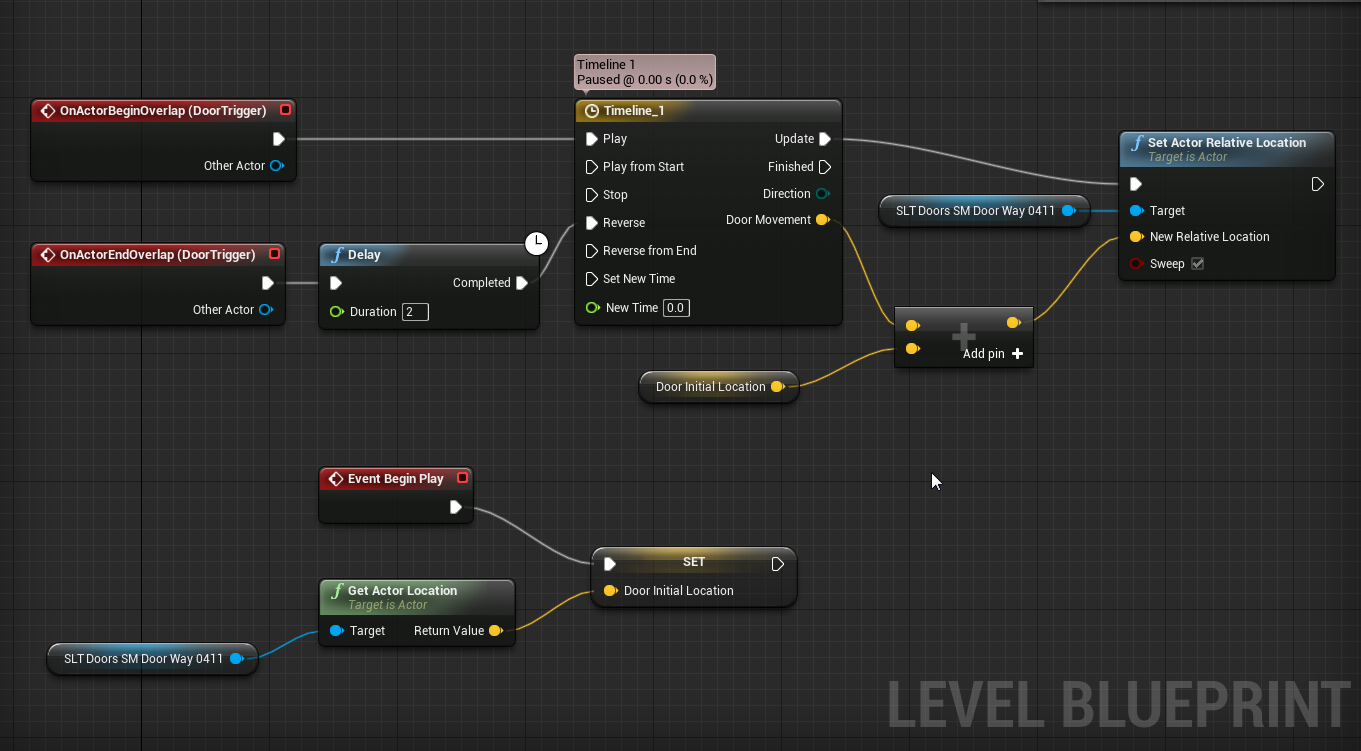
\includegraphics[width=0.5\textwidth]{OtherImages/UEBlueprint.png}
    \caption{Source: \url{https://docs.unrealengine.com/en-US/ProgrammingAndScripting/Blueprints/UserGuide/Timelines/Examples/OpeningDoors/index.html}}    \label{UnrealEngineBlueprint}

\end{figure}

\subsubsection{Unity}
Unity is currently the most commonly used game engine with over 2.5 million registered developers \cite{Unity_arnia_software}. Unity is developed by Unity Technologies and was first released in June 2005.  Over 60\% of augmented- and virtual reality games are created using Unity \cite{GameEngine_UnityGame_book}. 
\\~\\
Unity is free for personal and educational projects. To create the game, Unity allows a lot of features to be used through the GUI, but for full freedom, the creator would need to program in C\#. Unity however provides lots of resources to learn C\#. Unity also combines with Visual Studio where the IntelliSense can help with recommending functions to use as well as spot errors\footnote{\url{https://docs.microsoft.com/en-us/visualstudio/gamedev/unity/get-started/getting-started-with-visual-studio-tools-for-unity}}.


\subsection{Levels of Automation}
When talking about autonomous systems, it is important to know the different levels of autonomy. The modern day Tesla cars are level 3, which means they can be driven autonomously for the majority of the time, but do need a human driver as a fallback system \cite{teslaSelf, Bagloee2016}.
\begin{table}[H]
\begin{tabular}{lll}
\textbf{Level} & \textbf{Name}                   & \textbf{Description} \\
0     & No Automation          & The driver is solely controlling the vehicle\\
1     & Driver Assistance      & Cruise control is an example of this             \\
2     & Partial Automation     & Automatic parking            \\
3     & Conditional Automation & Modern day Tesla cars            \\
4     & High Automation        & Vehicle almost fully automated           \\
5     & Full Automation        & Vehicle never needs human input
\end{tabular}
\caption{Source: \url{https://link.springer.com/article/10.1007/s40534-016-0117-3\#Sec3}}
\end{table}

For this project all our simulations will be level 5. 

\subsection{Mixed Traffic Simulation}
The purpose of a mixed traffic simulation is to model the interaction between different types of agents, for example the the interaction between pedestrians, autonomous robots and vehicles. This is important because having a fully automated agent has to interact with a lot more than only other fully automated agents \cite{KernerBorisS2021Eoad}. 
\\~\\
A mixed traffic simulator can be used to simulate different situations where an autonomous system has to react to other agents behavior. This will mean the implemented algorithm will have the opportunity to try out a lot more complex scenarios a lot faster than in real life. This will help speed up development time. 


\subsection{API}
API stands for Application Programming Interface. This will allow a program to communicate with one-another. The API will define what kind of requests another program can make, how to make them, and the what the format should be. APIs also need to be documented so that other developers know how they work \cite{WulfJochen2020FVCw}.
\\~\\
In the case of our simulators, APIs will be used to communicate between an external program and the simulator itself. These communications could contain information for how to control the agent, or it could contain information from what the agent observes. 

\subsection{Digital Twin}

\subsection{Reinforcement Learning}

\subsection{Imitation Learning}

\subsection{Blender}
%Training machine learning models will be mentioned a few times when looking at the simulators.